\documentclass[14pt,final,titlepage,pscyr]{hedwork}
\usepackage[russian]{babel}
\usepackage[utf8]{inputenc}
\usepackage[derivative]{hedmaths}
\usepackage{graphicx}
\usepackage{array}
\usepackage{listings}
\usepackage{hyperref}

\graphicspath{{images/}}
\renewcommand{\vec}[1]{\mathbf{#1}}

\lstdefinelanguage{OpenCL}{morekeywords=
	{__kernel,kernel,__local,local,__global,global,% 
		__constant,constant,__private,private,% 
		char2,char3,char4,char8,char16,% 
		uchar2,uchar3,uchar4,uchar8,uchar16,% 
		short2,short3,short4,short8,short16,% 
		ushort2,ushort3,ushort4,ushort8,ushort16,% 
		int2,int3,int4,int8,int16,% 
		uint2,uint3,uint4,uint8,uint16,% 
		long2,long3,long4,long8,long16,% 
		ulong2,ulong3,ulong4,ulong8,ulong16,% 
		float2,float3,float4,float8,float16,% 
		image2d_t,image3d_t,sampler_t,event_t,% 
		bool2,bool3,bool4,bool8,bool16,% 
		half2,half3,half4,half8,half16,% 
		quad,quad2,quad3,quad4,quad8,quad16,% 
		complex,imaginary},% 
}% 

\faculty{Факультет электроники и вычислительной техники}
\department{<<Электронно-вычислительные машины и системы>>}
\subject{Вычислительные системы и сетевые технологии}
\topic{Решение системы ОДУ методом Рунге-Кутты 4 порядка}
\variant{9}
\student[m]{студент группы САПР-1.1п\\Голубев~А.~В.}
\teacher[m]{доцент технических наук\\Андреев~А.~А.}

\begin{document}
\maketitle
\tableofcontents
\section{Постановка задач}
	\begin{enumerate}
		\item Реализовать с использованием технологий параллельных вычислений задание по вариантам 
			(минимум 2 технологии: MPI и OpenMP, CUDA и OpenMP, OpenMP / OpenCL, Xeon Phi + MPI, 
			MPI / GridGain, cloud computing и т.д.)
		\item Оценить ускорение, степень параллелизма и другие параметры своих реализаций. Построить 
			таблицы и графики на основании тестирования (в зависимости от числа узлов / ядер и от 
			размерности задачи).
		\item Пройти он-лайн тестирование по курсам (\url{www.intuit.ru}): С.А. Немнюгин Основы MPI и 
			Введение в облачные вычисления 
	\end{enumerate}

\section{Параллельная реализация явного метода Рунге-Кутты}
	Метод Рунге -- Кутты позволяет получать одношаговые разностные схемы различного порядка точности, в 
	которых в зависимости от точности выбранной формулы правая часть системы может на рассматриваемом шаге 
	вычисляется несколько раз.

	Для построения вычислительных схем методов Рунге -- Кутты четвёртого порядка в тейлоровском разложении 
	искомого решения \( \vec{y}(t) \) учитываются члены, содержащие степени шага \( h = t_{m+1} - t_m \) до 
	четвёртой включительно, наиболее часто используемой из которых является следующая:
	\begin{equation}
		\vec{y}_{m+1} = \vec{y}_m + \frac{\left( \vec{k}_1 + 2\vec{k}_2 + 2\vec{k}_3 + \vec{k}_4 \right)}{6}
		\label{eq8.9}
	\end{equation}
	где 
	\begin{gather}
		\vec{k}_1 = h\vec{f}\left(t_m, \vec{y}_m \right), \notag \\
		\vec{k}_2 = h\vec{f}\left(t_m + \frac{h}{2}, \vec{y}_m + \frac{\vec{k}_1}{2} \right), \notag \\
		\vec{k}_3 = h\vec{f}\left(t_m + \frac{h}{2}, \vec{y}_m + \frac{\vec{k}_2}{2} \right), \notag \\
		\vec{k}_4 = h\vec{f}\left(t_m + h, \vec{y}_m + \vec{k}_3 \right). \notag
	\end{gather}

	Схема \eqref{eq8.9} на каждом шаге \( h \) требует четырёх последовательных вычислений правой части 
	системы ОДУ для определения значений \( \vec{k}_1, \vec{k}_2, \vec{k}_3, \vec{k}_4 \).

	Поскольку в описанной выше вычислительной схеме наиболее трудоёмкой является операции расчёта правых 
	частей ОДУ при вычислении \( \vec{k}_i (i = 1, 2, 3, 4) \), то основное внимание следует уделить 
	распараллеливанию этой операции. Будем применять поход декомпозиции уравнений системы ОДУ на подсистемы. 
	Поэтому для инициализации рассмотрим следующую схему декомпозиции данных по имеющимся процессорным 
	элементам с локальной памятью: на каждый \( \mu \)-й ПЭ \( \mu = 0, \ldots, p - 1 ) \) распределяется 
	\( n/p \) дифференциальных уравнений и вектор \( \vec{y}_0 \in \mathbb{R}^n \). Далее расчёты 
	производятся по следующей схеме:
	\begin{enumerate}
		\item на каждой ПЭ одновременно вычисляются \( n/p \) соответствующих компонент вектора 
			\( \vec{k}_1 \) по формуле 
			\[ \left[ \vec{k}_1 \right]_\mu = h\left[ \vec{f}(t_m, \vec{y}_m) \right]_\mu; \]
		\item для обеспечения второго расчётного этапа необходимо провести сборку вектора \( \vec{k}_1 \) 
			целиком на каждом ПЭ. Затем независимо выполняется вычисление компонент вектора \( \vec{k}_2 \) 
			по формуле 
			\[ 
				\left[ \vec{k}_2 \right]_\mu = 
					h\left[ 
						\vec{f}(t_m + \frac{h}{2}, \vec{y}_m + \frac{\vec{k}_1}{2}) 
					\right]_\mu; 
			\]
		\item проводится сборка вектора \( \vec{k}_2 \) на каждом ПЭ, вычисляются компоненты вектора 
			\( \vec{k}_3 \): 
			\[ 
				\left[ \vec{k}_3 \right]_\mu = 
				h\left[ 
					\vec{f}(t_m + \frac{h}{2}, \vec{y}_m + \frac{\vec{k}_2}{2}) 
				\right]_\mu; 
			\]
		\item проводится сборка вектора \( \vec{k}_3 \) на каждом ПЭ, вычисляются компоненты вектора 
			\( \vec{k}_4 \):
			\[ \left[ \vec{k}_4 \right]_\mu = h\left[ \vec{f}(t_m, \vec{y}_m + \vec{k}_3 ) \right]_\mu; \]
		\item рассчитываются с идеальным параллелизмом компоненты вектора \( \vec{y}_{m+1} \) : 
			\[
				\left[ \vec{y}_{m+1} \right]_\mu = \left[ \vec{y}_m \right]_\mu + \frac{1}{6}\left( 
					\left[ \vec{k}_1 \right]_\mu + 2\left[ \vec{k}_2 \right]_\mu + 
					2\left[ \vec{k}_3 \right]_\mu + \left[ \vec{k}_4 \right]_\mu
				\right)
			\]
			и производится сборка вектора \( \vec{y}_{m+1} \) на каждом ПЭ. Если необходимо продолжить 
			вычислительный процесс, то полагается \( m = m + 1 \) и осуществляется переход на пункт 1.
	\end{enumerate}

	Заметим, что в данном алгоритме производится четыре операции вычисления вектора правых частей ОДУ, 
	шестнадцать операций сложения векторов и умножения вектора на число и четыре операции глобальной 
	сборки векторов. 

	В случае, когда \( \vec{f}(t, \vec{y}(t)) \equiv A \times \vec{y}(t) \), где 
	\( A \in \mathbb{R}^{n\times n} \) -- матрица с постоянными коэффициентами, можно получить алгоритм, 
	который имеет меньшее число межпроцессорных пересылок данных на одной итерации метода Рунге -- Кутты. 
	Для этого построим оператор перехода для одного вычислительного шага, позволяющий определить 
	значение вектора неизвестных на следующей итерации \( \vec{y}_{m+1} \) через \( \vec{y}_m \). 
	Преобразуем значения \( \vec{k}_1, \vec{k}_2, \vec{k}_3, \vec{k}_4 \):
	\begin{gather}
		\vec{k}_1 = hA\vec{y}_m, \notag \\
		\vec{k}_2 = hA\left(\vec{y}_m + \frac{\vec{k}_1}{2}\right) = 
			\vec{k}_1 + \left(\frac{h}{2}\right)A\vec{k}_1 = 
			\left( E + \left(\frac{h}{2}\right)A \right)\vec{k}_1 = 
			h\left( E + \left(\frac{h}{2}A \right)A \right) \vec{y}_m, \notag \\
		\vec{k}_3 = hA\left( \vec{y}_m + \frac{1}{2}\vec{k}_2 \right) = 
			\vec{k}_1 + \left( \frac{h}{2} \right)A\vec{k}_2 = 
			\vec{k}_1 + \left( \frac{h}{2} \right)A\left( \vec{k}_1 + 
			\left( \frac{h}{2} \right)A\vec{k}_1 \right) = \notag \\ =
			h\left( E + \left( \frac{h}{2} \right)A + \left( \frac{h}{2} \right)^2 A^2 \right)A\vec{y}_m, 
		\notag \\
		\vec{k}_4 = hA\left( \vec{y}_m + \vec{k}_3 \right) = 
			\vec{k}_1 + \left( hA + \left( \frac{h^2}{2} \right)A^2 + 
				\left( \frac{h^3}{4} \right)A^3 \right)\vec{k}_1 = \notag \\ = 
			h\left( E + hA + \left( \frac{h^2}{2} \right)A^2 + 
				\left( \frac{h^3}{4} \right)A^3 \right)A\vec{y}_m
		\notag
	\end{gather}
	и, подставив из в \eqref{eq8.9}, получим
	\begin{gather}
		\vec{y}_{m+1} = B\vec{y}_m; \quad
		B = E + hA\left( E + \left( \frac{h}{2} \right)A\left( 
			E + \left( \frac{h}{3} \right) A \left( E + \left( \frac{h}{4} \right)A \right) 
		\right) \right)
		\label{eq8.10}
	\end{gather}
	где \( B \) -- оператор перехода.

	Рассчитав заранее матрицу \( B \), получим вычислительный алгоритм, в котором каждое новое значение 
	вектора \( \vec{y}_{m+1} \) определяется за один шаг умножения матрицы \( B \) на вектор.

	При параллельной реализации \eqref{eq8.10} умножение блочных строк матрицы \( B \) на вектора 
	\( \vec{y}_m \) будет проводиться одновременно и независимо. Потребуется только после каждого 
	вычислительного шага по \eqref{eq8.10} проводить сборку вектора \( \vec{y}_{m+1} \) на всех процессорных 
	элементах.\cite{methods}

\section{Используемый пример}
В качестве примера используем СОДУ для расчёта направления силовых линий для различных векторных 
полей. Систему уравнений можно записать следующим образом:

\[
	\vec{A}(\vec{0}) = \vec{r}_0, \quad \cfrac{d\vec{r}}{dt} = \vec{A}\left( \vec{r}(t) \right)
\]

где \( \vec{A}(\vec{r}) \) -- векторное поле, \( \vec{r}(t) \) -- интегральная кривая, 
\( \vec{r}_0 \) -- начальное условие.

\newpage

\section{Используемое оборудование}
\noindentТестирование программ производилось на следующем оборудовании:
\begin{enumerate}
	\item AMD Opteron(TM) Processor 6272 @ 2.10Ghz x 64
	\item Intel(R) Core(TM) i5-4690 CPU @ 3.50GHz x 4
	\item GIGABYTE Radeon R9 280X @ 1.10Ghz [4.1 TFlops]
\end{enumerate}

\noindentИспользуемые операционные системы:
\begin{enumerate}
	\item CentOS release 6.5 (Final) / Linux version 2.6.32-431.el6.x86\_64
	\item Arch Linux / Linux 3.17.6-1-ARCH x86\_64
\end{enumerate}

\noindentИспользуемые версии компиляторов:
\begin{enumerate}
	\item gcc version 4.4.7 20120313 (Red Hat 4.4.7-11) (GCC)
	\item gcc version 4.9.2 20141224 (prerelease) (GCC) 
\end{enumerate}

\noindentФлаги оптимизации скомпилированных программ:
\begin{enumerate}
	\item -O3 -m64 -march=bdver1 -mavx -msse -msse2 -msse3 -msse4 -msse4.1 \\
		-msse4.2 -msse4a -mssse3 -mfpmath=387,sse -pipe
	\item -O3 -m64 -march=haswell -mavx -mavx2 -mmmx -mmovbe -msse \\
		-msse2 -msse3 -msse4 -msse4.1 -msse4.2 -mssse3 -mfpmath=sse,387 \\
		-Ofast -flto -funroll-loops -fomit-frame-pointer -pipe
\end{enumerate}

\newpage

\section{Последовательная программа}
Параллельная и последовательная программа реализованы в качестве заменяемого ядра. Исходный код ядер для 
последовательной (default) и параллельных (thread, OpenMP, OpenCL) программ представлены в разделе 
Приложение \eqref{sec:app}.

Результаты проведенных тестов представлены в разделе \ref{sec:test}. 

\section{Оценка алгоритма}
Время последовательного алгоритма для одного уравнения при реализации метода Рунге -- Кутта может быть 
описано следующим соотношением:
\[
	T_1 = s\cdot T_f + N \cdot \left[ s^2 \cdot t_\text{умн} + s^2 \cdot t_\text{сл} + 
		s \cdot T_f \right] + s \cdot t_\text{умн} + s \cdot t_\text{сл}
\]
где \( T_f \) -- время вычисления функции \( f \) -- правой части исходного дифференциального уравнения;
\( t_\text{умн} \) -- время выполнения операции одиночного умножения; \( t_\text{сл} \) -- время 
выполнения операции одиночного сложения; \( N \) -- число итераций в методе. Для представленного алгоритма 
время выполнения на \( p \) процессорах без учёта обменов и других накладных расходов задаётся соотношением:
\[
	T_p = T_f + N \cdot \left[ s \cdot t_\text{умн} + s \cdot t_\text{сл} + T_f \right] + 
		t_\text{умн} + t_\text{сл}
\]

Соответственно, коэффициент ускорения равен
\[
	S_p = \frac{T_1}{T_p} = \frac{s\cdot T_f + N\cdot\left[ 2s^2 \cdot t* + s\cdot T_f\right] + 2s\cdot t*}
			{T_f + N\cdot\left[ 2s\cdot t* + T_f\right] + 2\cdot t*}
\]
При подсчёте коэффициента ускорения будем считать, что \( t_\text{сл} = t_\text{умн} = t* \) -- любая 
арифметическая операция с плавающей точкой выполняется за одно и то же время независимо от вида операции.
Коэффициент ускорения для сложных функций правой части коэффициент ускорения практически равен числу 
процессоров:
\[
	S_p \approx \frac{s \cdot T_f + N \cdot s \cdot T_f}{T_f + N \cdot T_f } = s = p
\]

Тогда показатель эффективности будет равен:
\[
	E_p = \frac{T_1(n)}{pT_p(n)} = \frac{1}{p}S_p(n) = 1
\]

Оценим максимальное достижимое ускорение по закону Густавсона -- Барсиса:
\begin{equation}
	g = \frac{\tau(n)}{\tau(n) + \pi(n) / p}
	\label{eq:gusbar}
\end{equation}
здесь \( \tau(n) \) и \( \pi(n) \) есть времена последовательной и параллельной частей выполняемых 
вычислений, т.е. 
\[
	T_1(n) = \tau(n) + \pi(n), \quad T_p = \tau(n) + \pi(n) / p
\]
Преобразуем \eqref{eq:gusbar} к следующему виду:
\[
	g = \left( 1 - \frac{p}{p+1} \right)\frac{T_1}{T_p} - \frac{p}{p+1}
\]
Используя ранее полученное значение для ускорения, получим значение достижимого ускорения:
\[
	g = \left( p - \frac{p^2}{p+1} \right) - \frac{p}{p+1}
\]

Используя формулу для ускорения масштабирования, подставляя полученный ранее коэффициент \( g \):
\[
	S_p = p + (1-p)\cdot g = p + p \left( 1 - p \right) \left( 1 - \frac{p}{p+1} \right) - 
		p\left( \frac{1-p}{p+1} \right)
\]

\begin{figure}[ht!]
    \center
    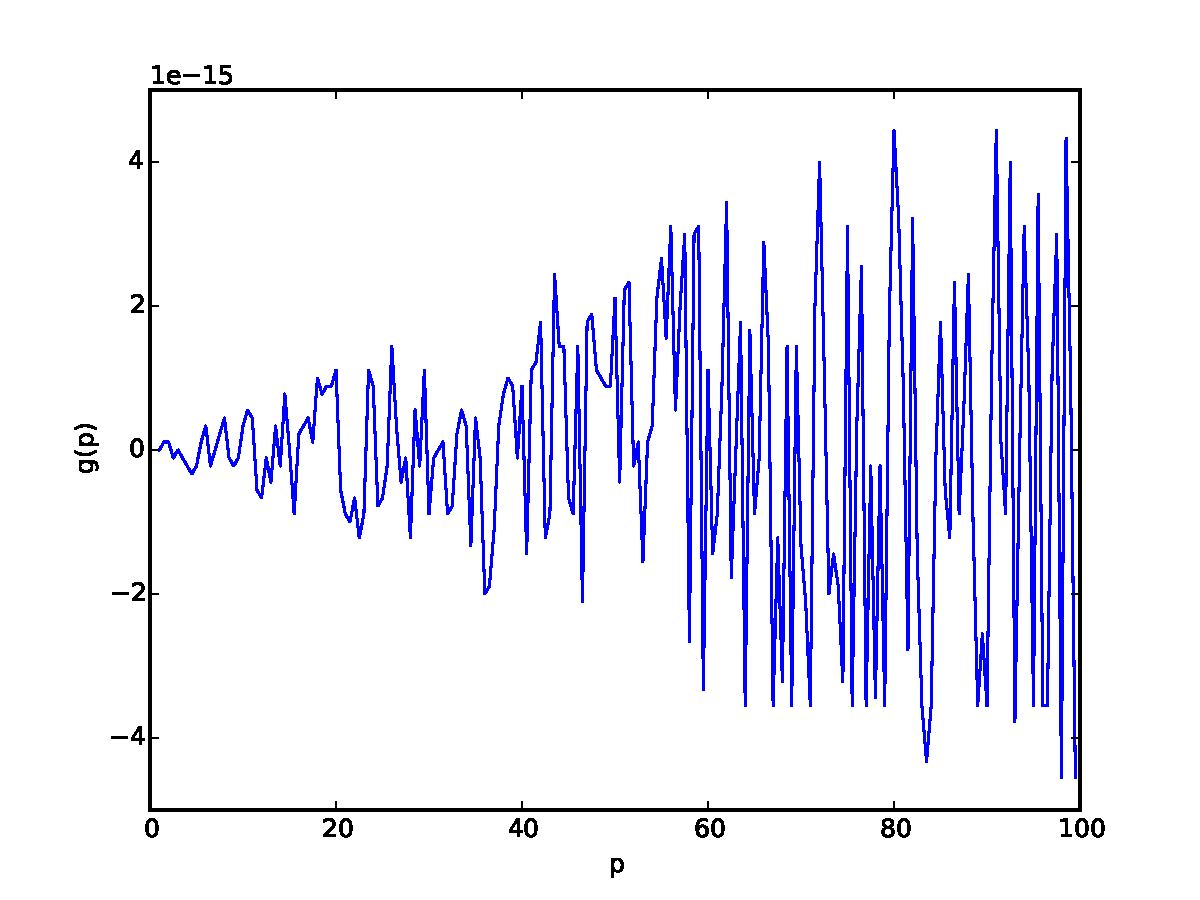
\includegraphics[width=0.7\textwidth]{g_p}
    \caption{Зависимость достижимого ускорения от количества процессорных элементов}
    \label{img:01}
\end{figure}

\newpage

\section{Входные данные}
	Тестирование последовательной и параллельной программы производился на следующем наборе данных
	\begin{table}[h]
		\begin{tabular}{|c|c|c|c|c|c|c|c|c|c|}
			\hline
			Шаг & \multicolumn{6}{c|}{Количество точек} & \multicolumn{3}{c|}{Данные} \\ \hline
			\( 10^{-8} \) & 100 & 1000 & 5000 & 10000 & 150000 & 200000 & lines & random & rotation \\ 
			\hline
			\( 10^{-16} \) & 100 & 1000 & 5000 & 10000 & 150000 & 200000 & lines & random & rotation \\ 
			\hline
		\end{tabular}
	\end{table}

	Программы для генерации входных данных доступны в конце приложения.

\newpage

\section{Результаты}
\label{sec:test}
Результаты полученные на кластере:
\begin{figure}[ht!]
    \center
    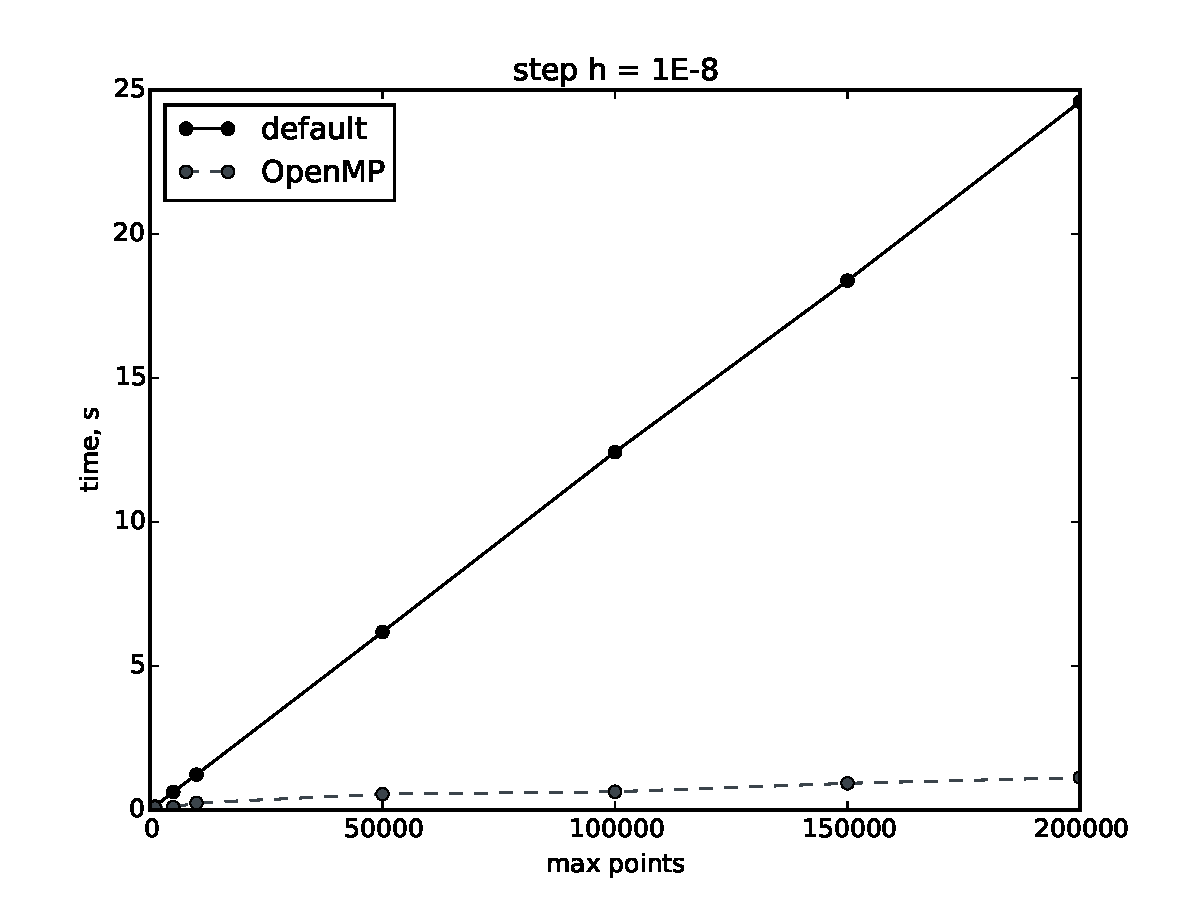
\includegraphics[width=0.8\textwidth]{linesField_cl_1E-8}
    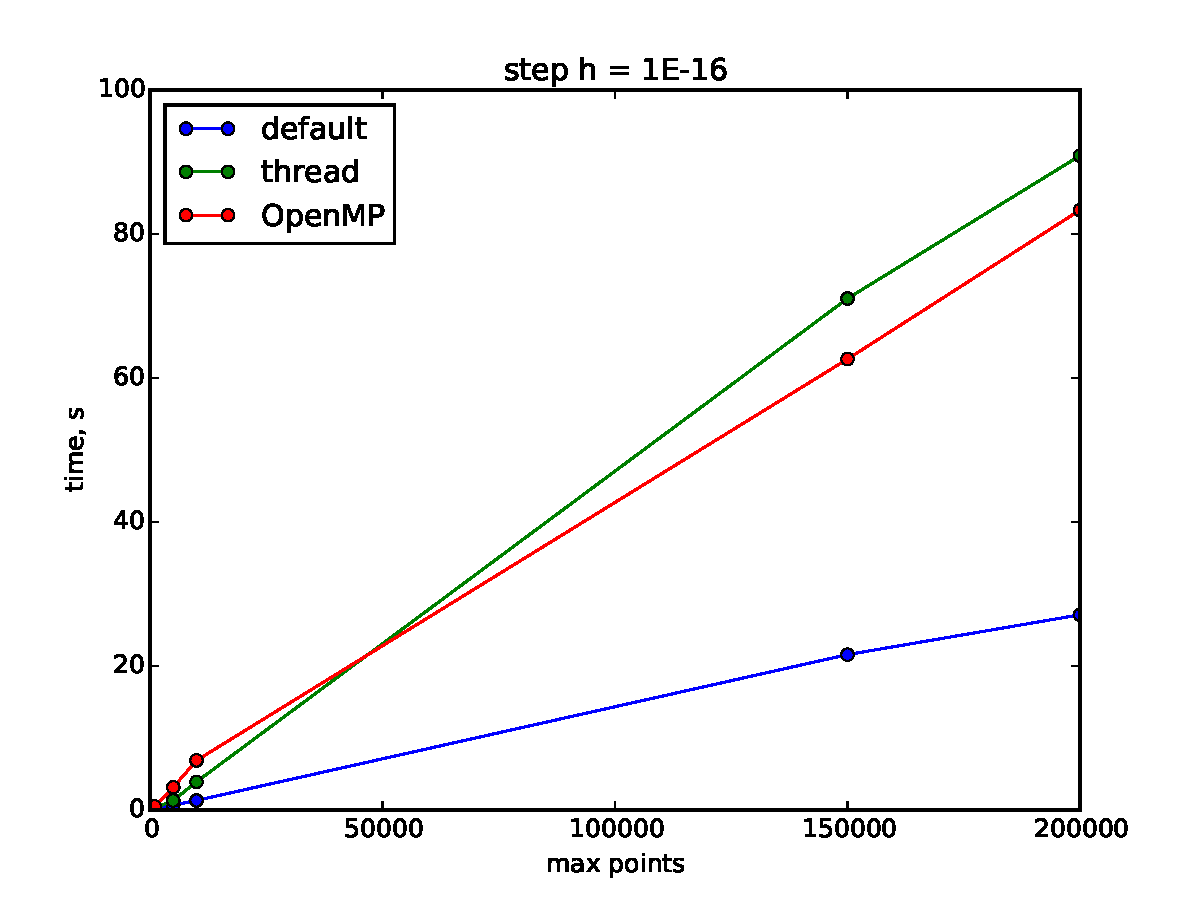
\includegraphics[width=0.8\textwidth]{linesField_cl_1E-16}
    \caption{linesField (256 вычислителей)}
\end{figure}

\pagebreak

\begin{figure}[ht!]
    \center
    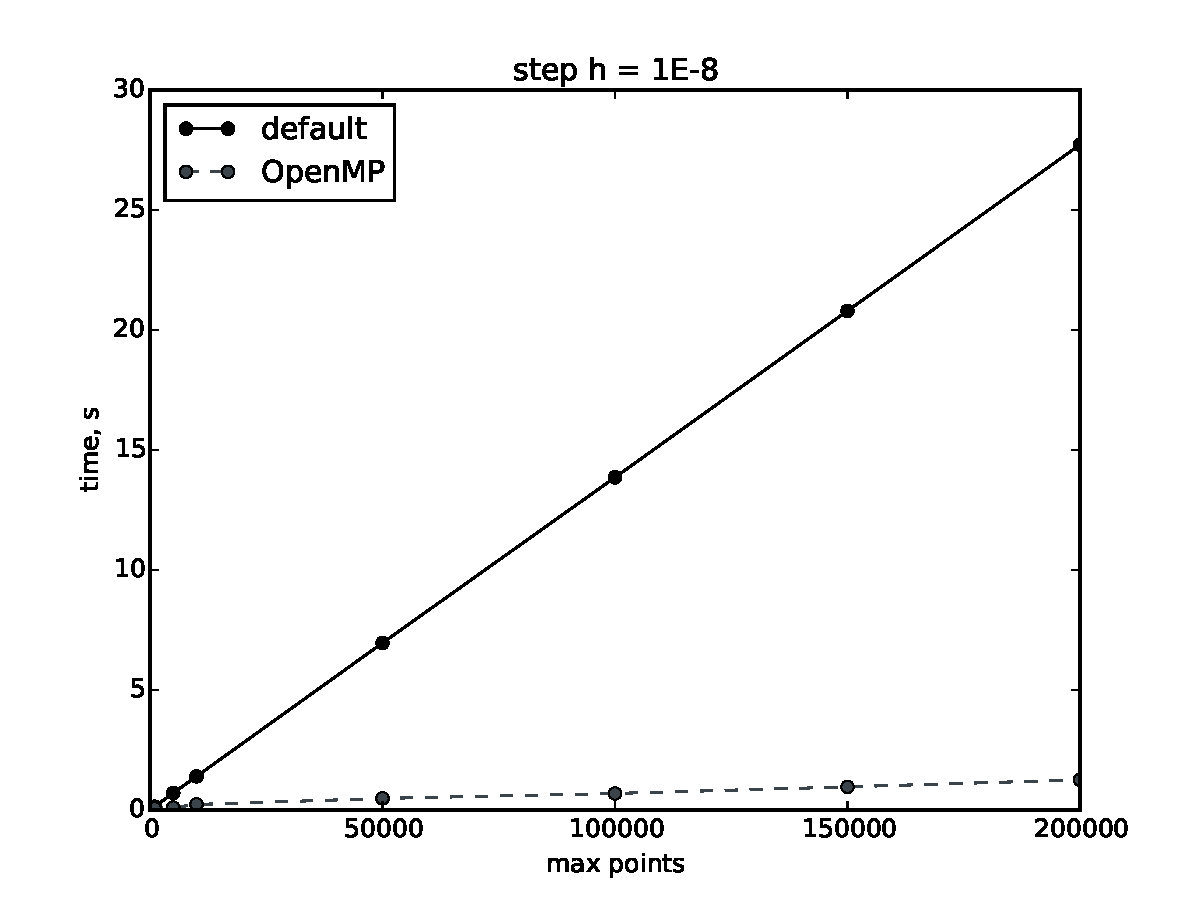
\includegraphics[width=0.8\textwidth]{randomField_cl_1E-8}
    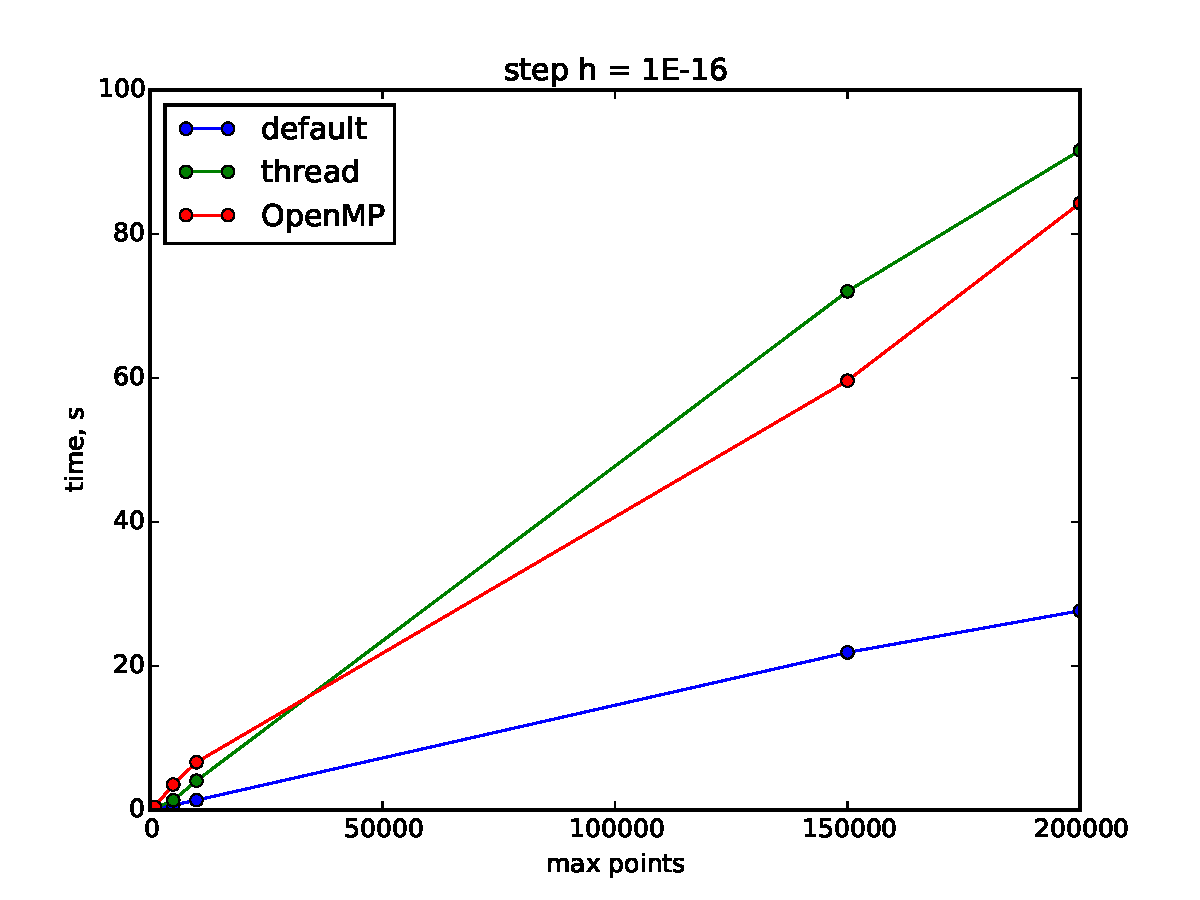
\includegraphics[width=0.8\textwidth]{randomField_cl_1E-16}
    \caption{randomField (256 вычислителей)}
\end{figure}

\pagebreak

\begin{figure}[ht!]
    \center
    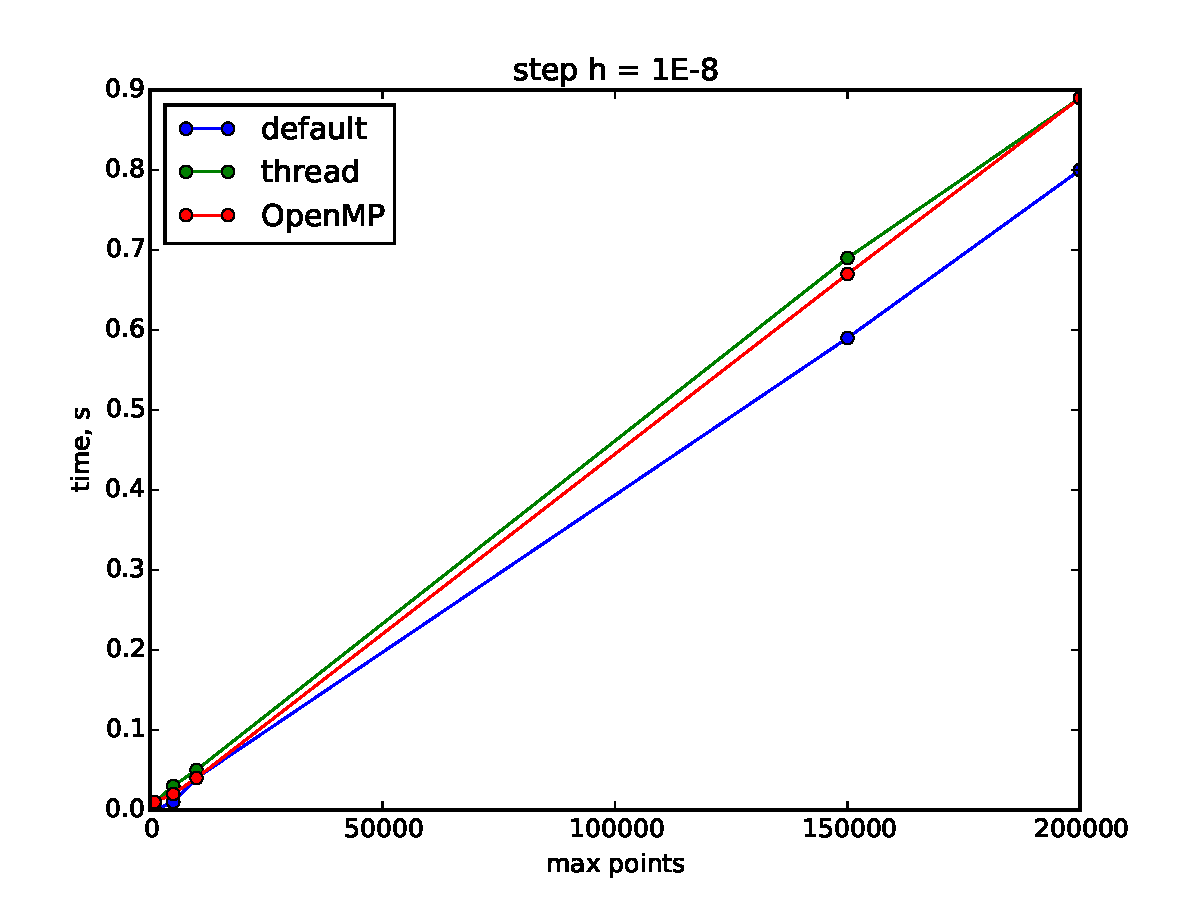
\includegraphics[width=0.8\textwidth]{rotationField_cl_1E-8}
    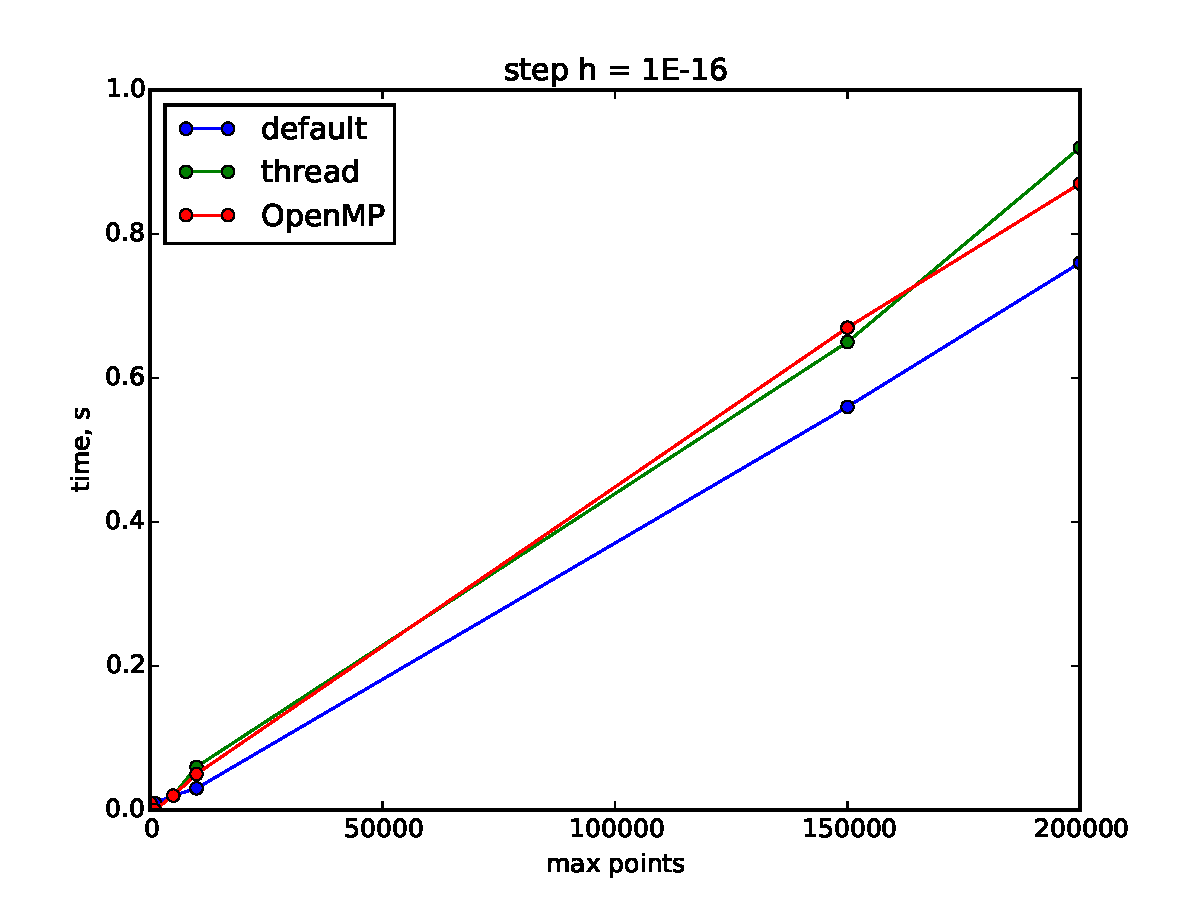
\includegraphics[width=0.8\textwidth]{rotationField_cl_1E-16}
    \caption{rotationField (7 вычислителей)}
\end{figure}

\pagebreak

Результаты полученные на стационарном компьютере:
\begin{figure}[ht!]
    \center
    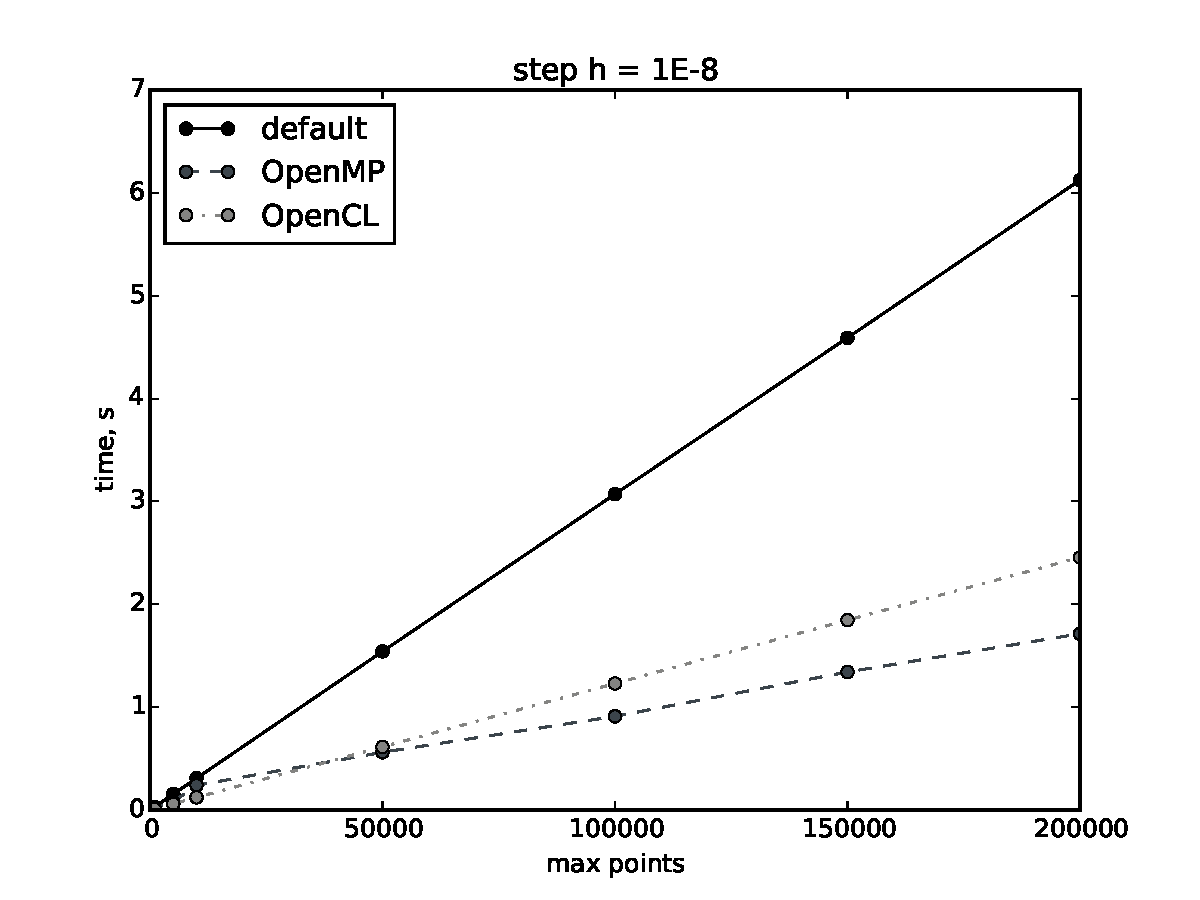
\includegraphics[width=0.8\textwidth]{linesField_my_1E-8}
    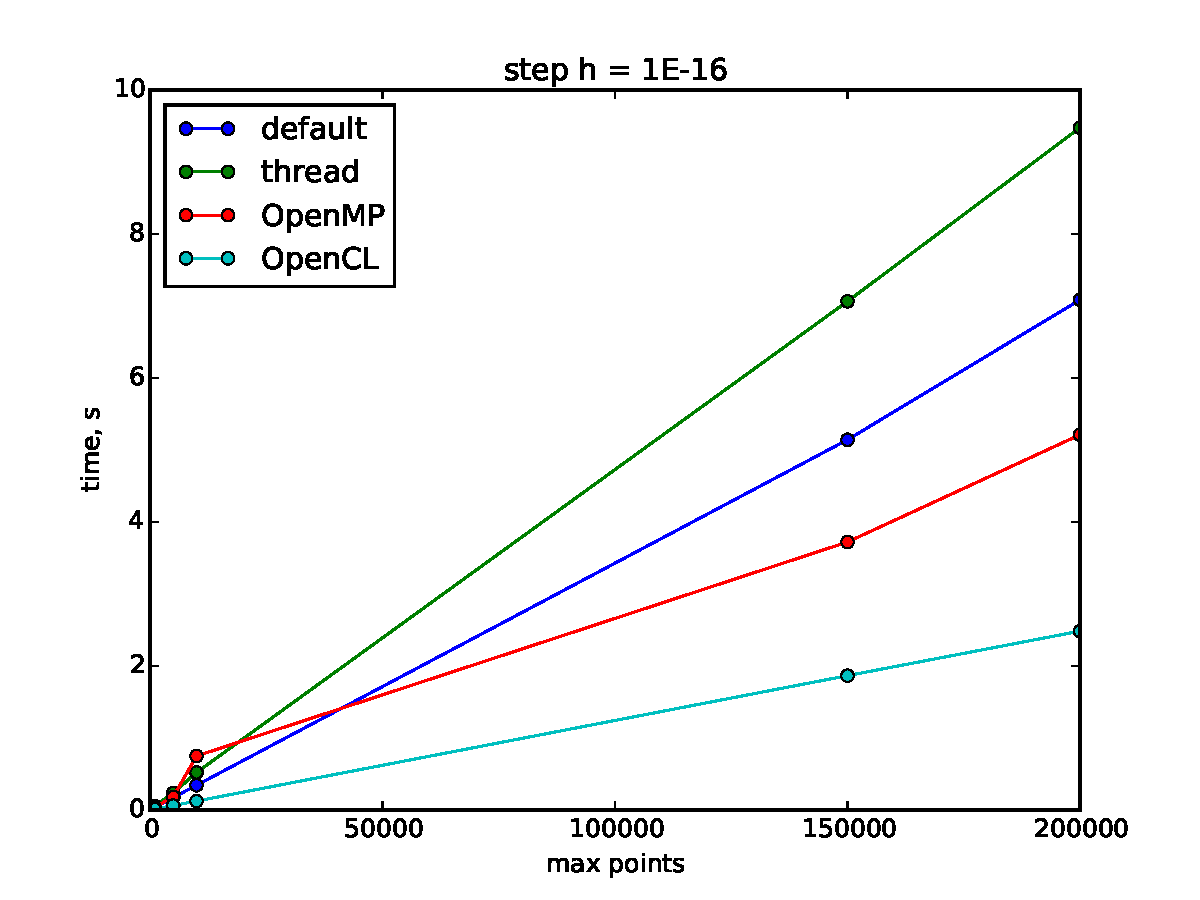
\includegraphics[width=0.8\textwidth]{linesField_my_1E-16}
    \caption{linesField (256 вычислителей)}
\end{figure}

\pagebreak

\begin{figure}[ht!]
    \center
    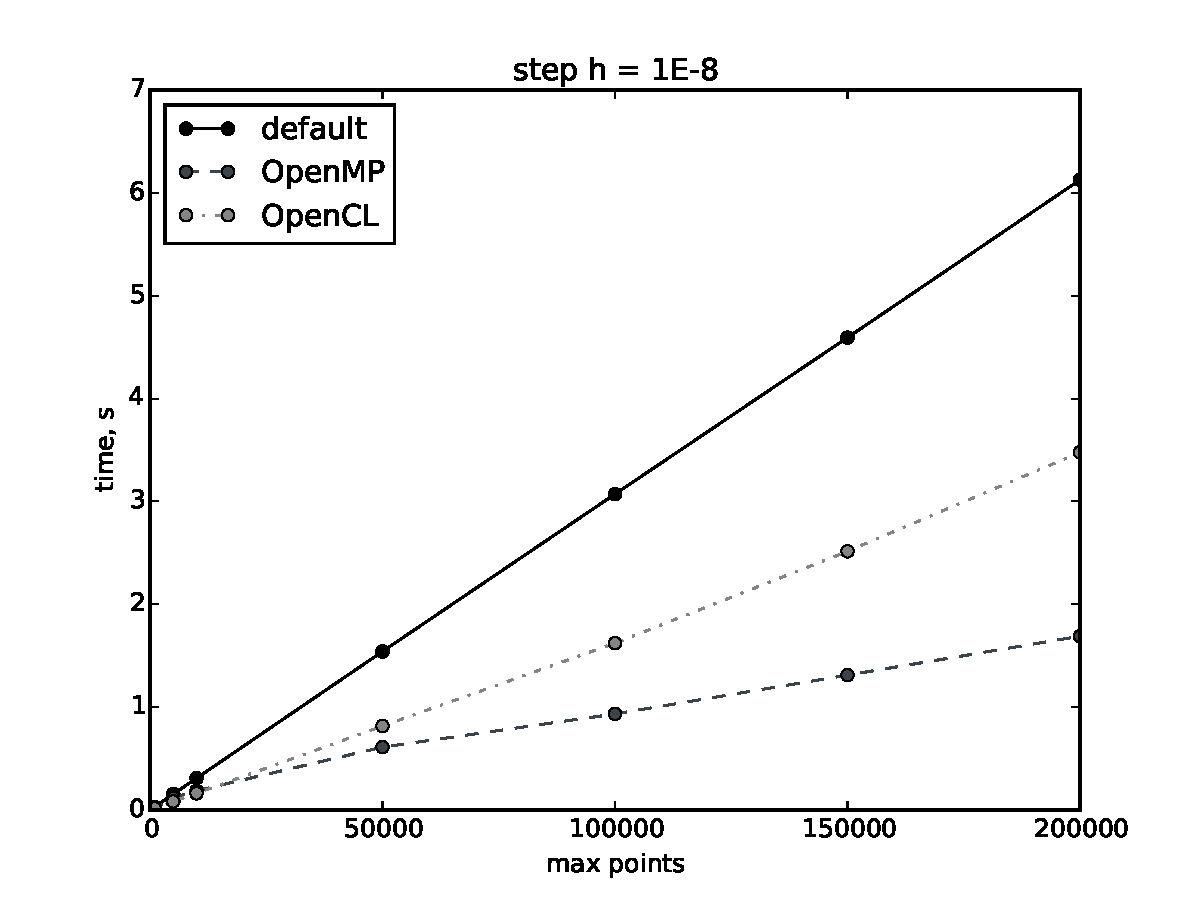
\includegraphics[width=0.8\textwidth]{randomField_my_1E-8}
    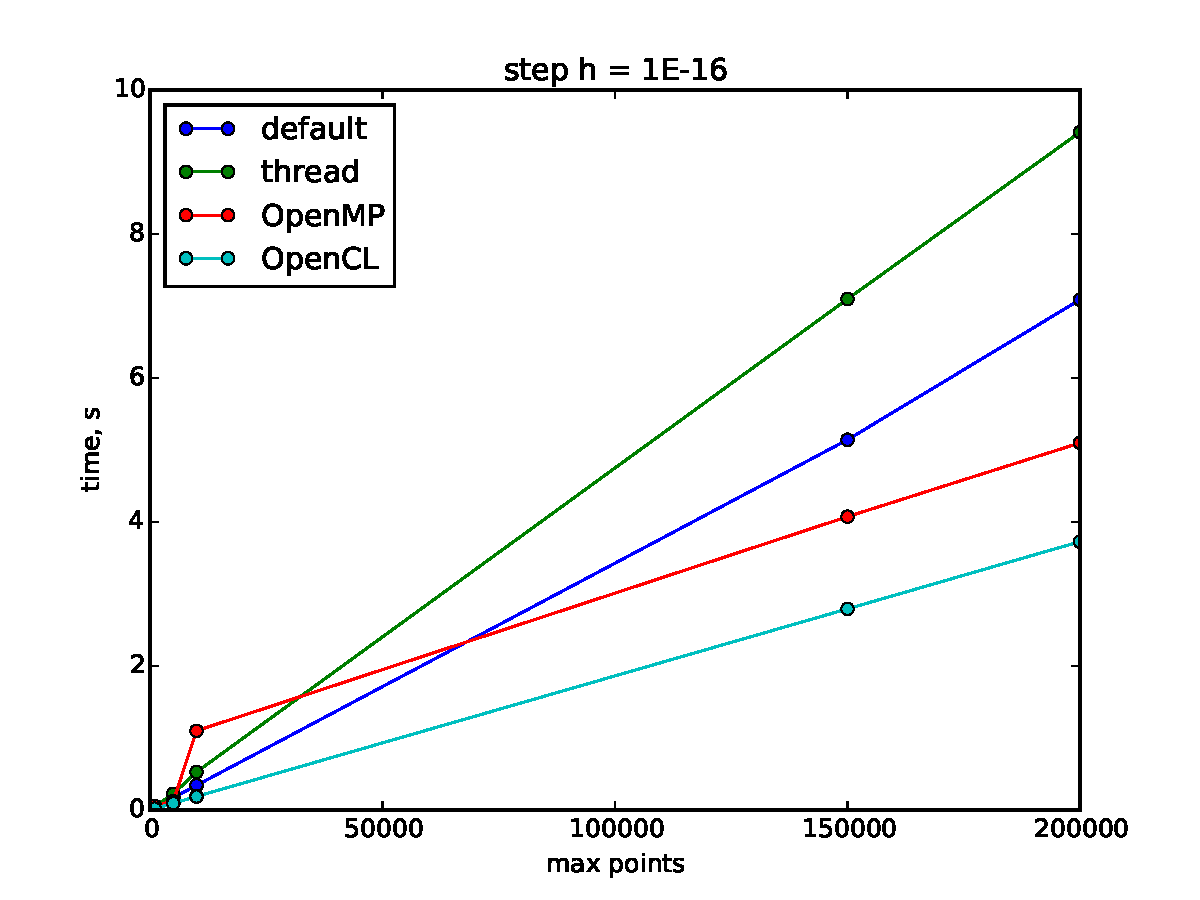
\includegraphics[width=0.8\textwidth]{randomField_my_1E-16}
    \caption{randomField (256 вычислителей)}
\end{figure}

\pagebreak

\begin{figure}[ht!]
    \center
    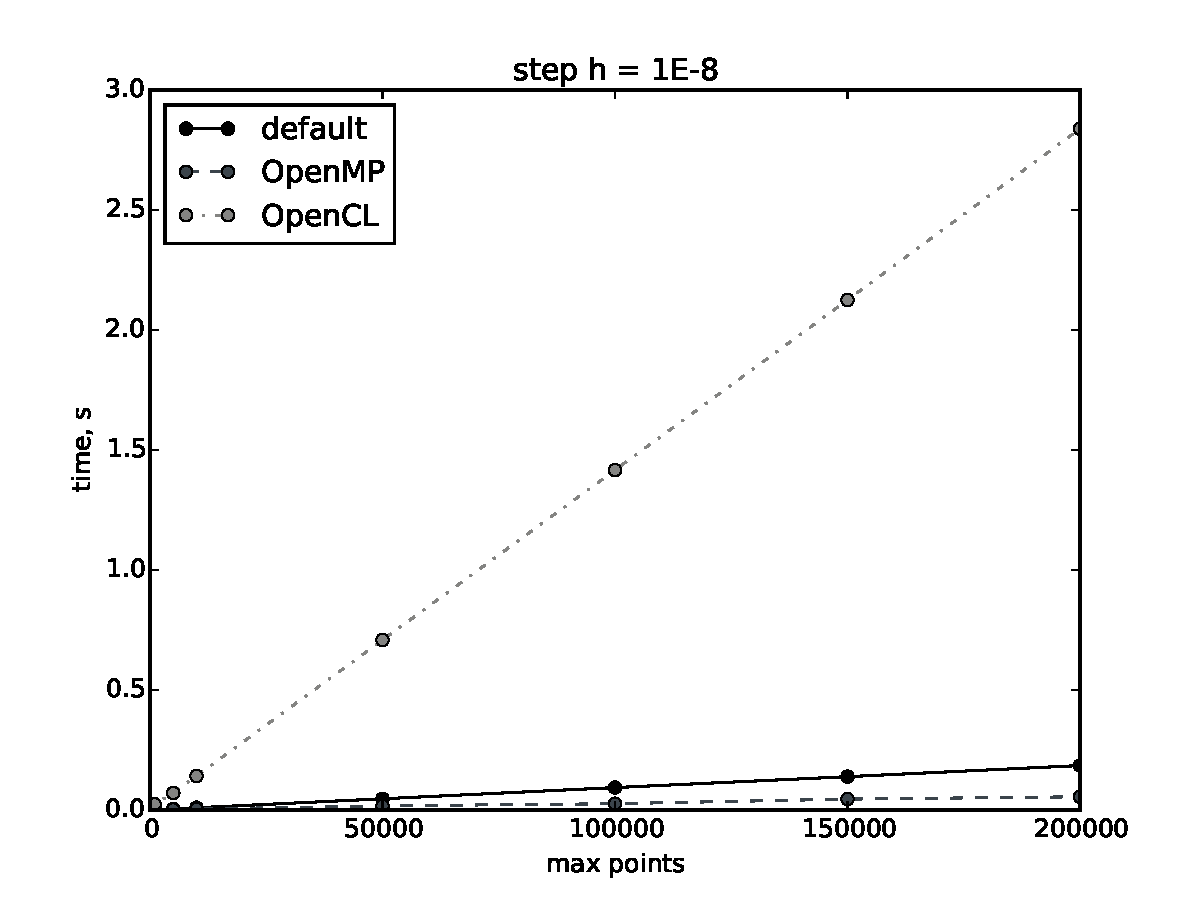
\includegraphics[width=0.8\textwidth]{rotationField_my_1E-8}
    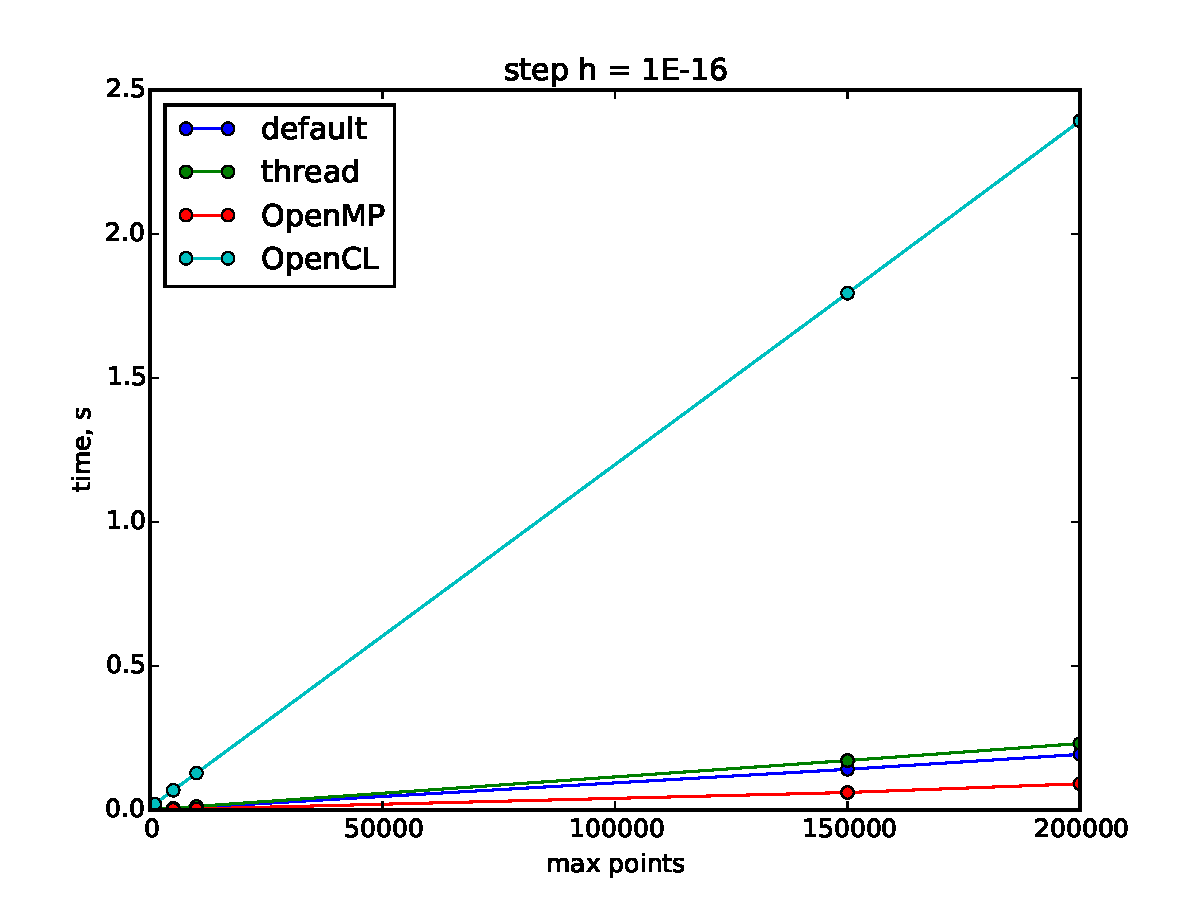
\includegraphics[width=0.8\textwidth]{rotationField_my_1E-16}
    \caption{rotationField (7 вычислителей)}
\end{figure}

\newpage

\section{Выводы}
В данной работе был рассмотрел параллельный алгоритм Рунге -- Кутты, произведена оценка его эффективности 
и получены экспериментальные данные на нескольких наборах данных.

Деградацию скорости вычислений на кластере можно объяснить рисунком \ref{img:01}, где достижимое 
ускорение резко осциллирует. Напротив, тесты проведённые на стационарном оборудовании показали хорошие 
результаты. Версии программ использующие OpenMP и OpenCL показали значительный прирост в скорости работы, 
при увеличении рассматриваемого интервала. Увеличение точности вычислений не сильно сказалось на скорости 
работы программ. Последний из примеров показал плохую работу OpenCL при малом количестве вычислительных 
блоков, что было ожидаемо, т.к. основное время расходуется на пересылку и сбор данных, а при малой 
сложности задачи это является критическим параметром.

\newpage

\renewcommand{\bibname}{Список используемой литературы}
\addcontentsline{toc}{section}{Список используемой литературы}
\begin{thebibliography}{10}
	\bibitem{methods} Cтарченко, А.~В. Методы параллельных вычислений~/ А.~В. Старченко, В.~Н. Берцун ~// 
		Томский государственный университет "--- 2013
	\bibitem{theory} Назарова, И.~А. Параллельные полностью неявные методы численного решения жестких 
		задач для СОДУ~/ И.~А. Назарова ~// Донецкий национальный технический университет "--- 2005
	\bibitem{book01} Горелов, Ю.~Н. Численные методы решений обыкновенных дифференциальных уравнений 
		(метод Рунге -- Кутта) ~/ Ю.~Н. Горелов ~// Самарский университет "--- 2006
	\bibitem{book02} Баркалов, К.~А. Образовательный комплекс <<Параллельные численные методы>> ~/ 
		К.~А. Баркалов ~// Нижний Новгород "--- 2011
	\bibitem{book03} Clauß, M. Simulating the Spread of Epidemics in Real-world Trading Networks 
		using OpenCL ~/ Martin Clauß "--- 10.02.2012
\end{thebibliography}

\newpage

\addcontentsline{toc}{section}{Приложение}
\label{sec:app}
\centerОбщая часть для всех программ:
\lstinputlisting[language=C++, basicstyle=\tiny, firstline=12, lastline=109]{code/rk_kernel_default.cpp}

\newpage

Ядро последовательной программы:
\lstinputlisting[language=C++, basicstyle=\tiny, firstline=116]{code/rk_kernel_default.cpp}

\newpage

Ядро программы использующая OpenMP:
\lstinputlisting[language=C++, basicstyle=\tiny, firstline=117]{code/rk_kernel_openmp.cpp}

\newpage

Ядро программы использующая потоки:
\lstinputlisting[language=C++, basicstyle=\tiny, firstline=116]{code/rk_kernel_thread.cpp}

\newpage

Ядро программы использующая OpenCL:
\lstinputlisting[language=OpenCL, basicstyle=\tiny, firstline=116]{code/rk_kernel_opencl.cl}

Настройка и работа с OpenCL:
\lstinputlisting[language=C++, basicstyle=\tiny, firstline=8]{code/opencl_init.cpp}

Программы генерации входных данных:
\lstinputlisting[language=C, basicstyle=\tiny]{code/lines.c}
\lstinputlisting[language=C, basicstyle=\tiny]{code/random.c}
\lstinputlisting[language=C, basicstyle=\tiny]{code/rotation.c}

\end{document}
